% NOTE: Build merge.pdf with `pdftk ra.pdf iso.pdf cat output merge.pdf` to preserve chapters and links, don't use texexec!! 
\documentclass[a4paper,pagesize,openany,14pt,parskip=never]{scrbook}
\KOMAoptions{twoside=false}
\usepackage{tabularx}
\usepackage{float}
\usepackage{amssymb}
\usepackage{emptypage}
\usepackage{mathrsfs}
\usepackage{hyperref}
\usepackage{fontspec, newunicodechar}
\newfontfamily\cochin{Cochin LT Std}
\newfontfamily\baybayin{OpenBaybayin}
\newfontfamily\baybayinh[Style=Historic]{OpenBaybayin}
\newfontfamily\baybayinb[RawFeature={+ss02}]{OpenBaybayin}
\newfontfamily\textfrak{UnifrakturMaguntia}
\setmainfont{TeX Gyre Pagella}
\setsansfont{TeX Gyre Heros}
\DeclareTextFontCommand{\textfallback}{\baybayin}
\usepackage{svg}
\usepackage{graphicx}
\usepackage{xcolor}
\hypersetup{
    colorlinks,
    linkcolor={blue!50!black},
    citecolor={blue!50!black},
    urlcolor={blue!50!black}
}
\usepackage{cleveref}
\usepackage[inline]{enumitem}
\usepackage{pdfpages}
\crefformat{footnote}{#2\footnotemark[#1]#3}
\newcommand{\≈}{$\approx$}
\newcommand{\la}{{\baybayin ᜎ}}
\newcommand{\da}{{\baybayin ᜇ}}
\newcommand{\ra}{{\baybayin ᜍ}}
\newcommand{\ta}{{\baybayin ᜆ}}
\newcommand{\wa}{{\baybayin ᜏ}}
\newcommand{\ei}{{\baybayin ᜁ}}
\newcommand{\eicirc}{◌ᜒ{\baybayin \symbol{"1712}}}
\newcommand{\na}{{\baybayin ᜈ}}
\newcommand{\rizaleoRA}{{\baybayinb \symbol{"E005}}}
\newcommand{\hanunoo}{Hanun\'o\textquotesingle o}
\newcommand{\cochinQ}{{\cochin Q}}
%\setkomafont{author}{\scshape}
\let\cleardoublepage=\clearpage
\setkomafont{title}{\rmfamily\bfseries}
\usepackage{blindtext}
\title{The {\em baybayin} ``ra''---{\baybayin ᜍ}}
\author{Fredrick R. Brennan \\ <copypaste@kittens.ph>}

\titlehead{\begin{center}
  \makebox[0pt][c]{\smash{%
    \parbox[t][\dimexpr\textheight-\ht\strutbox\relax][b]{\textwidth}{%
        \centering
      \includesvg[width=0.5\textwidth]{RAU170D}
      }}}
\end{center}
  }

\subtitle{its origins and a plea for its formal recognition}
\dedication{{\small\em Special thanks to: \\
Deborah Anderson\footnote{Script Encoding Initiative/Universal Scripts Project, UC Berkeley}, for her much needed expertise and review \\
Renan Pagador, without whom this request would not have been possible \\
Jayson Villaruz, for his help in finding materials \\
Norman de los Santos, for his kind support of this proposal and expertise \\
\symbol{"200C}\\
And finally, all the staff at Ateneo de Manila University's Rizal Library for graciously allowing me to browse their Filipiniana archives \\
\symbol{"200C}} \\
\symbol{"200C}\\
\ra\ra\ra\ra \\
\symbol{"200C}\\
See with what large letters I am writing to you with my own hand! Galatians 6:11}
\begin{document}
\maketitle
\tableofcontents
\addchap{Introduction}
{\em Baybayin} is the local name for what the Unicode Standard calls the Tagalog block of the Basic Multilingual Plane (BMP). Proposed in 1998 by Michael Everson, four scripts were encoded at once: Tagalog, \hanunoo, Buhid and Tagbanwa.

At the time of encoding, only ancient documents were considered for the Tagalog script. As a result, the Tagalog `ra' was not encoded. 

However, as \hanunoo\ and Buhid included a `ra', and because all four scripts were encoded due to the same proposal, a spot was, in a splendid twist of fate, left open for a `ra' in Tagalog as well; although it was seemingly never intended for the use the community gave it.

This spot, U+170D, has become a {\em de facto} standard among {\em baybayin} writers in the Philippines and the Filipino diaspora. Several modern fonts, including the one that appears on Philippine currency to write the word {\em Pilipino}, use U+170D as a `ra'. (See \S\ref{Fonts}) Software, if it can output \ra, uses U+170D. (See \S\ref{Software}) Documents online, if they include \ra, most often have it encoded as U+170D.

This proposal is at once an extensive study on the {\em baybayin} `ra' and a plea for the Unicode consortium to recognize the {\em de facto} standard of the user community, and to legitimize U+170D as `ra', because some large tech companies, such as Google, patron of the Noto fonts, refuse to encode characters that the Unicode Standard does not recognize, hindering the development of {\em baybayin} and the community in using its script.

\section{Linguistic details}
The letter `da', {\baybayin ᜇ}, in Old Tagalog was known as {\em dara}. In his thesis,\footnote{{\em A study of the ancient Philippine syllabary with particular attention to its Tagalog version}, Joseph G. Lapallargas, Ateneo de Manila University, 1974, Z 115.5 T2 E76} Joseph G. Lapallargas writes: ``Contact with the Spanish and English and the consequent numerous borrowings have brought about some changes in the phonetic and phonemic structure of Tagalog. [\ldots] If formerly there were no prevocalic clusters in Tagalog, now they are of frequent occurrence. If [d] and [r] were submembers of a single phoneme, now the two are separate phonemes.'' {\baybayin ᜍ}, `ra', is required to write modern Tagalog or Filipino in the Tagalog ({\em baybayin}) script without introducing ambiguity into the text. This became apparent very early in the revival of the Tagalog script in the Philppines; the first known appearance of the Tagalog `ra' (Zambales form) appears in print in 1922.

Some contemporary users of the script are okay with the ambiguity introduced by the lack of a \ra\, using \da\ for Tagalog words and \la\ for Spanish words. However, in my examination of the evidence, the majority of the contemporary {\em baybayin} user community prefers to use \ra, and even if some users find it distasteful and would prefer only to use the original seventeen {\em baybayin} letters, they are free to do so. After all, I am not trying to prescribe the use of \ra\ to anyone, but merely to describe that \ra\ is being used frequently and therefore needs a codepoint.

\addchap{Unicode considerations}
\section{Characters}
I propose to encode only one character to cover all the modern variants discussed in this paper, to be encoded at U+170D and named \textsf{TAGALOG LETTER RA}. 

The Zambales form of the {\baybayin ᜍ}, {\baybayinh ᜍ}, is only found in historical texts and {\em could} be encoded as U+170D and selected in a font by using the OpenType feature \texttt{hist}, \textsf{Historical Forms}, as I've done in the OpenBaybayin font that I made to typeset this document. In {\em baybayin} text, {\baybayinh ᜍ} has exactly the same meaning as {\baybayin ᜍ}, and I found no texts where both were in use except the one I'm writing. I received some feedback from the Script Ad Hoc committee that ``It is graphically quite different from the RA you propose, though it has the same sound, so it should also be encoded.''

Therefore, out of respect to Script Ad Hoc, I also propose the Zambales {\baybayinh ᜍ} be encoded at U+171F and receive name \textsf{TAGALOG LETTER ZAMBALES RA}. In my discussions with users, it is of utmost importance to them that \textsf{TAGALOG LETTER RA} (\ra) be encoded, but many would also welcome \textsf{TAGALOG LETTER ZAMBALES RA} ({\baybayinh ᜍ}) to be able to transcribe historical texts in which it appears. The situation can be seen as analogous to that of \textsf{LATIN SMALL LETTER LONG S} (ſ) and \textsf{LATIN SMALL LETTER S} (s). Ultimately the decision is up to the Consortium.

The variants of the marked {\baybayin ᜇ} form of the letter {\baybayin ᜍ} are mere stylistic choices with equivalent meaning and can all be encoded in the same letter in the same way that Q, {\textfrak{Q}}, \textsf{Q}, \cochinQ, and $\mathscr{Q}$ can all be represented by \textsf{LATIN CAPITAL LETTER Q}, U+0051, with the style chosen being based on font. Indeed, as {\em baybayin} fonts are primarily made based on handwriting, it is unsurprising that there are so many variants; in the samples I observed, other letters had many variants as well; for example, at times \na\ would have a straight center line instead of the standard squiggly one in the \na\ used in this sentence.

I am aware of the following stylistic variants of the modern \ra:

\begin{enumerate}
    \item Generic --- \ra\ (\S\ref{Android}; \S\ref{Surat})
    \item Generic, longer stroke --- {\baybayinb \symbol{"E006}}\ (\S\ref{MB2018})
    \item Rizaleo --- \rizaleoRA\ (\S\ref{RizaleoC})
    \item Bikol --- {\baybayinb \symbol{"E004}}\ (\S\ref{BED})
    \item Applied to a cursive {\baybayinb \symbol{"E007}} --- {\baybayinb \symbol{"E008}}\ (\S\ref{Maharlika})
    \item\label{DoubleLoop} Double cursive loop --- {\baybayinb \symbol{"E009}}\ (\S\ref{Kalem})
\end{enumerate}

This is not meant to be an exhaustive listing, there are definitely variants beyond those that I have listed; rather it is meant to be a list of the major stylistic variants I've seen in reviewing works written in the {\em baybayin} script.

Some of these, especially \textnumero\ref{DoubleLoop}, are caused by attempting to write the {\em baybayin} script in a cursive form on pen and paper, which is not how it was traditionally written.

\section{Properties}
The proposed General Category properties for \textsf{TAGALOG LETTER RA} are:

\begin{verbatim}
170D;TAGALOG LETTER RA;Lo;0;L;;;;;N;;;;;
171F;TAGALOG LETTER ZAMBALES RA;Lo;0;L;;;;;N;;;;;
\end{verbatim}

\subsection{\texttt{NamesList.txt} character remark}

So end users and font designers better understand this glyph and its use, I propose that \textsf{TAGALOG LETTER RA} receive the following character note in \texttt{NamesList.txt}:

\begin{quote}
    Not used to write Old Tagalog.
\end{quote}

I propose that \textsf{TAGALOG LETTER ZAMBALES RA} receive the following character note in \texttt{NamesList.txt}:

\begin{quote}
    Not used to write Old Tagalog; historical form of TAGALOG LETTER RA.
\end{quote}

\section{Collation}

In the original proposal, Everson writes on pages three to four:

\begin{quote}
    UTR\#3 states: “The alphabetical order of Tagalog is known from Tagbanwa speakers and is described in folktales. This order is used in the accompanying charts. The two vowel signs are added at the end of the alphabet.” The names list in UTR\#3, however, is (except for the vowel signs) given in Latin alphabetical order ({\em a, i, u, ba, da, ga, ha, ka, la, ma, na, nga, pa, sa, ta, wa, ya, -i, -u}). Daniels \& Bright give another ordering, “based on the 16th-century Tagalog sequence” ({\em a, i, u, ha, pa, ka, sa, la, ra, ta, na, ba, ma, ga, da, ya, nga, wa}). This proposal gives the characters in the traditional Brahmic order ({\em a, i, u, ka, ga, nga, ta, da, na, pa, ba, ma, ya, ra, la, wa, sa, ha}), which is followed in many sources, including Santos 1994 and 1995.
\end{quote}

This having been the standard for more than twenty years, I see no reason to change it; this Brahmic Unicode order is used by software such as the JavaScript input method Lexilogos (\S\ref{Lexilogos}) and is the order that Norman de los Santos (\S\ref{Nordenx}) presents his fonts in. While some writers, such as Lloyd Zapantas (\S\ref{Lloyd}), use a Spanish-influenced collation,\footnote{That is to say, in order: {\baybayin ᜀᜊᜃᜇᜁᜄᜑᜎᜋᜈᜅᜂᜉᜍᜐᜆᜂᜏᜌ} (placement of {\baybayin ᜀᜁᜂ} may vary)} there is no reason in my opinion to change the standard collation to match.

Therefore, I request for the collation to be as follows, matching \hanunoo\ and Buhid:

\begin{quote}
    {\baybayin ᜌ} $>$ {\baybayin ᜍ} $>$ {\baybayin ᜎ}
\end{quote}

That is to say, {\baybayin ᜌ} comes before {\baybayin ᜍ} comes before {\baybayin ᜎ}. Assuming \ra\ is encoded, {\baybayinh ᜍ} should come after it, so:

\begin{quote}
    {\baybayin ᜍ} $>$ {\baybayinh ᜍ} $>$ {\baybayin ᜎ}
\end{quote}

\addchap{History}

\section{The Zambales `ra', {\baybayinh ᜍ}}

The first form of the {\em baybayin} `ra' is the Zambales `ra'. Its main source is the 1895 book {\em Estudio de los antiguos alfabetos Filipinos} by Cipriano Marcilla y Martin where it appears on page 23. 

\includegraphics[width=0.7\textwidth]{ZambalesAlphabet}

On page 34, its origin is explained thus (emphasis mine):

\begin{quote}
    En la p\'ag 23. y con el n\'um. 7 damos el alfabeto de Zambales escrito por un Agustino. En el archivo de S. Agustin hemos registrado este precioso documento del que por falta de medios no hemos podido sacar unfacsimile de las firmas que contiene. {\bfseries Seg\'un la portada se escribi\'o el 1601} y se lee en la \'ultima p\'agina en letra clara y escrita con tinta encarnada <<Este arte hall\'e tirado en el pueblo de Bolinao, quando estuve all\'i el a\~no de 1780. Fr. Agustin Maria.>>
\end{quote}

Translated quite literally:

\begin{quote}
    On page 23, in figure \textnumero7, we reproduce the Zambales alphabet as written by an Agustinian [monk]. In the archive of San Agustin we've inspected to this precious document, which through lack of means we were unable to make a facsimile of its signatures. {\bfseries According to the cover page, it was written in 1601} by an Agustinian [monk], and on the last page one can read in letters written clearly in red ink: ``I found this art in the town of Bolinao when I was there in the year 1780. Signed Fr. Agustin Maria.''
\end{quote}

In the latter years of the Spanish Empire's presence in the Philippines, interest in restoring {\em baybayin}, which had been surpressed by the Spanish and now lay only in history books, returned. Indeed, some revolutionary flags contained the {\em baybayin} letter `ka', {\baybayin ᜃ}, which stood for both {\em kalayaan} (freedom) and {\em katipunan} (the revolutionaries).\footnote{Alvarez, S.V., 1992, Recalling the Revolution, Madison: Center for Southeast Asia Studies, University of Wisconsin-Madison, ISBN 1-881261-05-0, p. 105} 

In 1922, Ignacio Borbon Villamor took an interest in the restoration of the {\em baybayin} script, but quickly realized that the Tagalog language had changed too much due to Spanish influence, in his book, {\em La antigua escritura filipina}, he recommends using the Zambales `ra':

\includegraphics[width=0.7\textwidth]{ZambalesRa1}

Translated into English:

\begin{quote}
    In the alphabet of Zambales, taken, according to P. Marcilla, from a 1601 manuscript, we find the letter R written as {\baybayinh ᜍ}, so that, if we wish to correctly write ``America'', we would write it as {\baybayinh ᜀᜋᜒ\kern-0.2emᜍᜒᜃ}.
\end{quote}

The community of {\em baybayin}/Tagalog script revivalists happily received this advice mid-century---most documents of the era which include `ra' use the Zambales `ra'. Many of these publications are hard to come by as they had limited production runs and before the internet were costly to produce, but I was able to find some in the Ateneo de Manila University's Rizal Library:
\newpage
\subsection{Mariano Dario Canseco's {\em Palatitikan kayumanggi} (1966)}
{\baybayinh ᜍ} can be seen clearly in the words {\baybayinh ᜐᜍᜒᜎᜒ}---{\em sarili}, {\baybayinh ᜃᜓᜍᜓᜃᜓᜍᜓ}---{\em kurukuro} and {\baybayinh ᜀ\kern-0.2emᜍᜏ}---{\em araw}.
 \\
\includegraphics[width=0.9\textwidth]{PK}

\newpage
Includes some dictionary entries that show {\baybayinh ᜍ}

\includegraphics[width=0.5\textwidth]{Dict}

In the edition in the archives of the Rizal Library, the following handwritten note can be found which uses {\baybayinh ᜍ}:

\includegraphics[width=0.7\textwidth]{HandwritingZ}

{\baybayinh ᜑᜈᜇᜓᜄ ᜅ ᜋᜌ ᜀᜃᜇ ᜐ ᜋᜃᜆᜅ ᜀᜋᜇᜓ ᜑᜒᜍᜈᜈᜇᜒᜐ} Hunyo 2, 1966

Handog ng may akda sa makatang Amado Hernandez. Hunyo 2, 1966

This is a gift from the author to the poet Amado Hernandez. June 2, 1966

\subsection{{\em Panitik Silangan}, September 1963}
\includegraphics[width=0.9\textwidth]{PS}

{\baybayinh ᜍ} can be seen in many words in this short-lived newsletter, for example, {\baybayinh ᜁᜒᜇᜒᜆ\kern-0.2emᜍᜌᜎ}, {\em editoryal} and {\baybayinh ᜐᜍᜒᜎᜒᜅ}, {\em sariling}.

\newpage
\section{The modern `ra', {\baybayin ᜍ}}
\subsection{The Bikol `ra', {\baybayinb \symbol{"E004} } }
\label{BikolRa}
\subsubsection{{\em Bikol--English Dictionary}, 1986}
\label{BED}

Besides the Zambales `ra', there is another `ra' with a long pedigree, the so-called ``Bikol'' `ra'. This form of `ra' is so similar to the modern form that it could be called a minor variant form; in the same way the tail of the letter Q moves about depending on the style of the writer, the marked form of the {\baybayin ᜇ} moves about, finding itself sometimes as {\baybayinb \symbol{"E004}} and other times {\baybayin \symbol{"170D}}, but for completeness I include it anyway.

%\begin{figure}[h]
%    \centering
%    {
%    \includesvg[width=0.25\textwidth]{Q}
%    }\raisebox{3em}{\footnotemark}
%    {
%    \fontsize{47pt}{48pt}\selectfont
%    {\baybayin \symbol{"170D}} {\baybayinb \symbol{"E004}} {\baybayinb \symbol{"E005}}
%    }\raisebox{1em}{\footnotemark}
%\end{figure}
%\addtocounter{footnote}{-2}
%\stepcounter{footnote}\footnotetext{Source: \href{https://commons.wikimedia.org/wiki/File:Q\_typographic\_styles.svg}{Wikimedia Commons}, Psi\^hedelisto, 3 February 2017}
%\stepcounter{footnote}\footnotetext{The third {\baybayin \symbol{"170D}} shown here, {\baybayinb \symbol{"E005}}, is the Rizaleo `ra'. See \S X}

Despite being called by the word Bikol, which is an area of Luzon, the original chart which shows this form of the {\em baybayin} `ra' doesn't mention Bikol at all, (although it should be noted that Camarines is in the Bicol region), and is found in an old Tagalog--English dictionary held by the Madrid National Library. It's marked {\em Caracteres antiguos con los que escribían estos naturales del Tagalog y Camarines}, ``Ancient characters with which these natives of the Tagalogs and Camarines used to write''.\footnote{The full text of the work can be seen at \url{http://bdh.bne.es/bnesearch/detalle/bdh0000044798}} The version shown below is as reprinted in the 2004 edition of Malcolm Warren Mintz's {\em Bikol--English Dictionary}.

\includegraphics[width=0.7\textwidth]{oldbikol3}
\newpage
The 1986 edition of the {\em Bikol--English Dictionary} features a stylized Bikol {\baybayinb \symbol{"E004}} on its cover.

\includegraphics[width=0.7\textwidth]{DCover}
\newpage


Computers and the internet brought the {\em baybayin} community closer together, making it much easier and cheaper to print {\em baybayin} materials. 

\subsection{{\em Rizaleo} `ra'---{\baybayinb \symbol{"E005}}}
\subsubsection{Marius V. Diaz's {\em Aklat Sanayan ng Abakadang Rizaleo}, 1994}
The first truly modern `ra' appears in the book {\em Aklat Sanayan ng Abakadang Rizaleo} (Exercise Book for the Rizal Alphabet) by Marius V. Diaz. This work details a slightly stylized {\em baybayin} alphabet and shows off several Type 1 computer fonts\footnote{According to the book's text, all the font styles shown in the book were available as Type 1 fonts in 1994, but due to the age of the work, the obsolescence of the format, and the existence of better Unicode fonts, the fonts no longer seem to be distributed online.} made by Diaz to write (his slightly modified version of) {\em baybayin}.

\begin{figure}[h]
\includegraphics[width=0.7\textwidth]{AR_PRS}
\end{figure}

\newpage
All the styles in the book are named after Jos\'e Rizal, so the {\baybayin ᜍ} can be clearly seen in all of them:\footnote{Except in the words {\em Rizaulo} and {\em Rizanayan}, which are misprinted---the beginning {\baybayin ᜍᜒ} is missing.}

\begin{figure}[H]
\includegraphics[width=0.7\textwidth]{Rizal-fontsF}
\end{figure}
\newpage
\label{RizaleoC}
Diaz was also a calligrapher, and included this calligraphy in the book. It is almost the same as typical modern {\em baybayin}, except Diaz marks the vowel `a' with a line above, which to my knowledge no other {\em baybayin} does.

\begin{figure}[H]
\includegraphics[width=0.5\textwidth]{ARCalligraphy}
\end{figure}
The calligraphy, a quote by Jos\'e Rizal, reads:

    {\baybayin ᜀᜅ᜔ ᜑᜒᜈ᜔ᜇᜒ ᜎᜓᜋᜒᜅᜓᜈ᜔ ᜐ ᜉᜒᜈᜅ᜔ᜄᜎᜒᜈ᜔ᜄᜈ᜔ ᜀᜌ᜔ ᜑᜒᜈ᜔ᜇᜒ ᜋᜃᜍᜍᜆᜒᜅ᜔ ᜐ ᜉᜆᜓᜆᜓᜅᜓᜑᜈ᜔᜶}

    Ang hindi lumingon sa pinanggalingan ay hindi makakarating sa patutunguhan.

    He who does not look back to where he came from will never reach his destination.

\newpage
\addchap{Further evidence}
The modern Baybayin `ra', {\baybayin ᜍ}, is disseminated widely as of this writing in 2019. I will outline multiple lines of evidence for its existence and usage by the contemporary community as an argument for its encoding:

\begin{itemize}
    \item Printed materials;
    \item News articles;
    \item Tattoos;
    \item Signs;
    \item Art;
    \item Fonts;
    \item Software.
\end{itemize}

\section{Printed materials}

As the modern `ra' is contemporary to the internet and the spread of Facebook in the Philippines, there is not as much printed material as may be expected. However, with the gracious help of the community, I was able to find a number of examples which will hopefully satisfy the Consortium.

\subsection{Jeremiah Cordial's {\em The Seventh Moon}, 2018}

This fantasy novel has {\em baybayin} sayings on the heading of every chapter. In many of them, the modern \ra\ can be clearly seen. For example, chapter \textnumero47 has this saying attached:

%\begin{figure}[h]
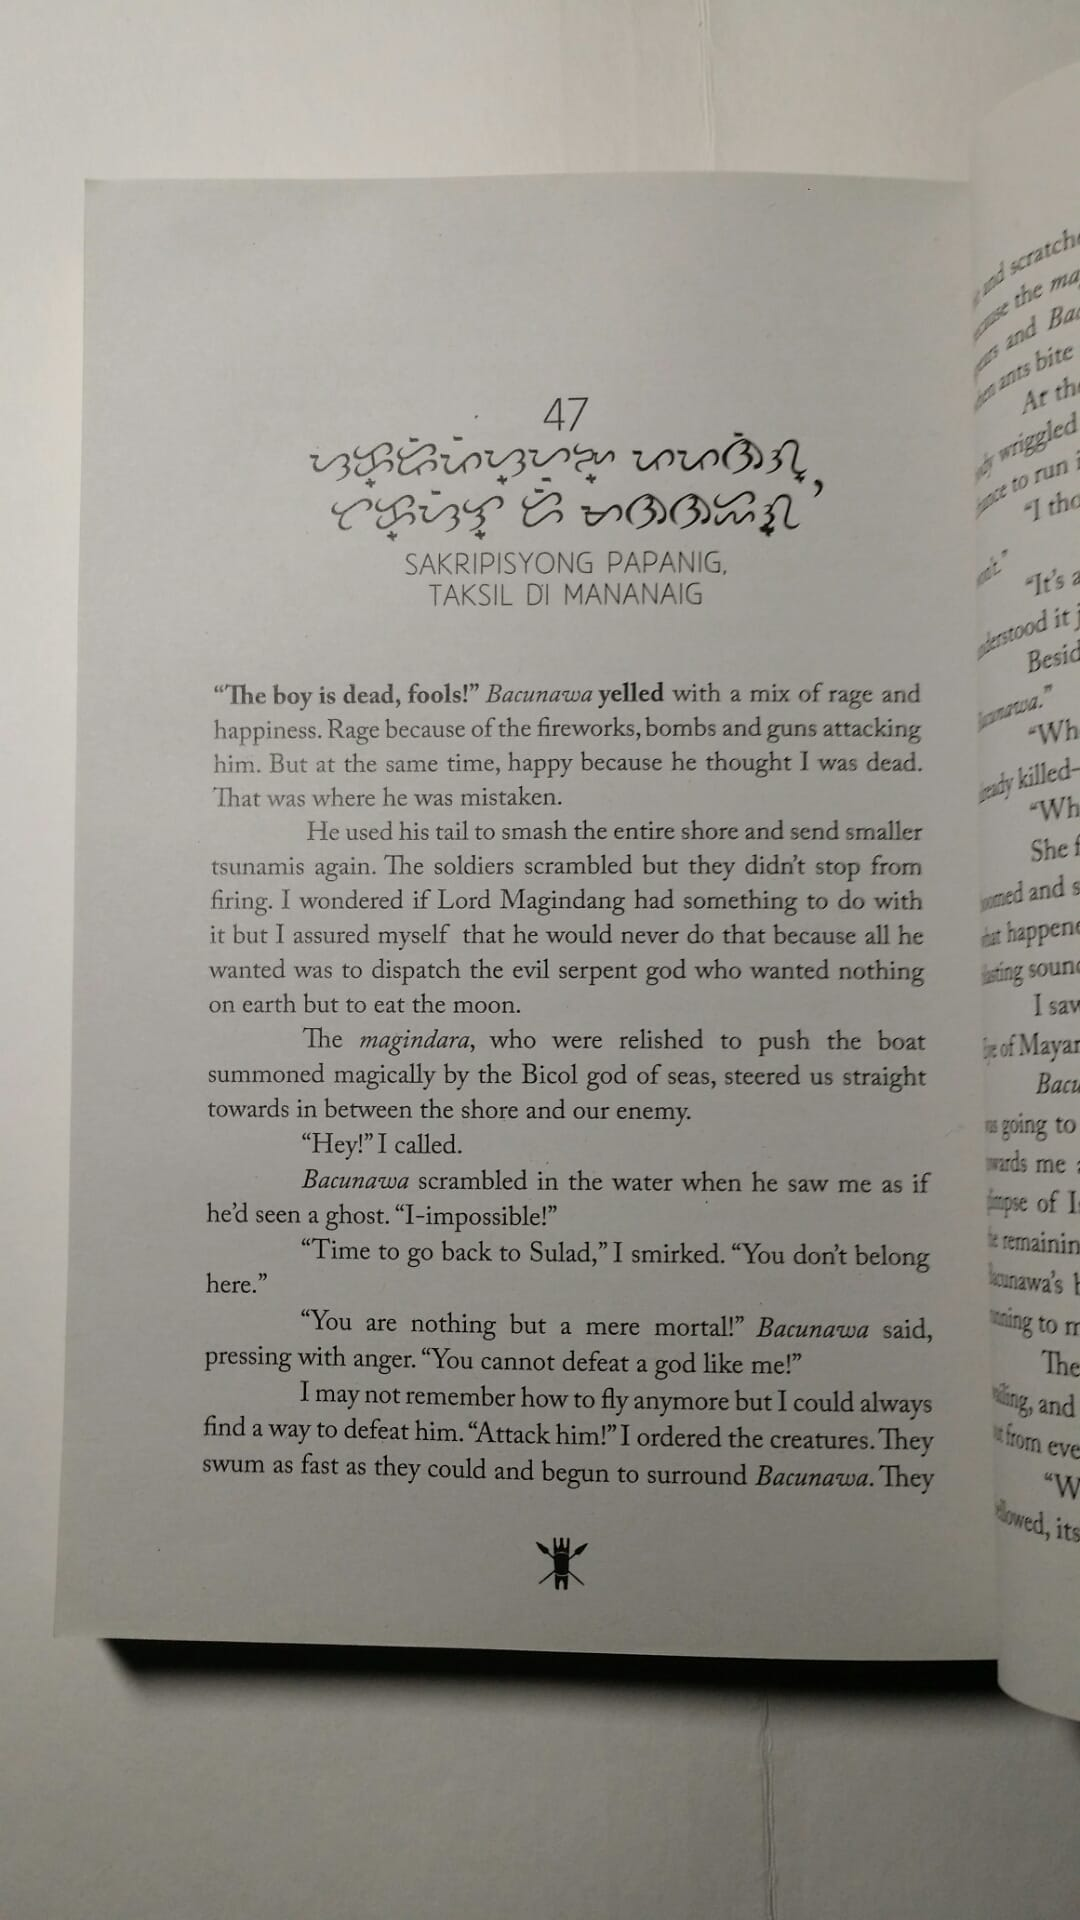
\includegraphics[width=0.5\textwidth]{7thMoon}
%\end{figure}

Transcribed: {\baybayin ᜐᜃ᜔ᜍᜒᜉᜒᜐ᜔ᜌᜓᜅ᜔ ᜉᜉᜈᜒᜄ᜔}, {\baybayin ᜆᜃ᜔ᜐᜒᜎ᜔ ᜇᜒ ᜋᜈᜈᜁᜄ᜔}

Tagalog: Sakripisyong papanig, taksil di mananaig

English (loosely): One [should] favor sacrifice, so traitors don't prevail

\subsection{Jean-Paul G. Potet's {\em Bayb\'ayin: L\textquotesingle Alphabet Syllabique des Tagals}, 2012 (French edition)}

The modern {\baybayin ᜍ} can be found on page {181} in a rather unusual example. It is an English sentence written semi-phonetically in {\em baybayin}. {\baybayin ᜍ} can be seen in the word {\baybayin ᜀᜍᜒ}, {\em are}.
 \\
%\begin{figure}[h]
\includegraphics[width=0.5\textwidth]{Potet2}
%\end{figure}

\subsection{{\em Kalem (Anak Bathala)}, №1, 2013, BHM Publishing, graphic novel}
\label{Kalem}

The modern {\baybayin ᜍ} can be found all throughout this book; notably on the cover to transcribe the name of two of its authors, Bernard Mo{\bfseries r}illo and Edsel Af{\bfseries r}ica.

\includegraphics[width=0.6\textwidth]{MorilloAfrica}

Transcribed: {\baybayin ᜋᜓᜍᜒᜎ᜴ᜌᜓ} $\bigstar$ {\baybayin ᜀᜉ᜴ᜍᜒᜃ}

On occasion when the characters in the book speak, they also speak in {\em baybayin} which contains the {\baybayin ᜍ}. As an example of {\em baybayin} use, and {\baybayin ᜍ} use, among the characters, see this bubble on page 19:

\includegraphics[width=0.6\textwidth]{KalemSpeechBubble}

Transcribed: {\baybayin ᜑᜒᜈ᜴ᜇᜒ ᜃᜓ ᜀᜎᜋ᜴ ᜃᜓᜅ᜴ ᜊᜃᜒᜆ᜴ ᜆᜌᜓ ᜈᜍᜒᜆᜓ ᜐ ᜇᜁᜄ᜴ᜇᜒᜄ᜴ ᜅ᜔ ᜋ᜔ᜅ ᜆᜂ᜵ ᜃᜓᜅ᜴ ᜊᜃᜒᜆ᜴ ᜇᜒᜆᜓ ᜆᜌᜓ ᜉᜒᜈᜇᜎ ᜈᜒ ᜇᜒᜆᜒᜈᜓᜐ᜴᜶ ᜅᜓᜈᜒᜆ᜴ ᜑᜊᜅ᜴ ᜈᜍᜒᜆᜓ ᜆᜌᜓ᜵ ᜋᜄ᜴ᜎᜍᜓ ᜀᜃᜓ᜶}

Tagalog: Hindi ko alam kung bakit tayo narito sa daigdig ng mga tao, kung bakit dito tayo pinadala ni Detinos. Ngunit habang narito tayo, maglalaro ako.

English: I don't know why we're here on this Earth of the humans, or why Detinos brought us here. But as long as we're here, I'll play around.

\subsection{Kristian Kabuay's {\em Surat Magazine}, \textnumero 1, December 2018}
\label{Surat}

The publication of this magazine was funded by a Kickstarter\footnote{\url{https://www.kickstarter.com/projects/baybayin/surat-1st-magazine-using-an-endangered-script-in-5/posts/2342594}---Kabuay rose \$3,136 and wrote of the magazine: {\em The inaugural Surat (to write) Magazine will be mainly written using indigenous writing systems in the Philippines in multiple languages covering topics from culture, art, poetry, food, fashion, travel, etc.}} and was billed as ``The first of it's kind in over 50 years."

The magazine is multilingual, however there is a long section written in the Tagalog {\em baybayin} script which includes our friend, the letter {\baybayin ᜍ}, in numerous instances. I will transcribe a line found on page 58 just as an example.

\begin{figure}[H]
\includegraphics[width=0.7\textwidth]{SURAT_Ef}
\end{figure}

Transcription: {\baybayin ᜈᜅ᜴ ᜈᜃᜒᜆ ᜀᜅ᜴ ᜋᜄᜈ᜴ᜇᜅ᜔ ᜉᜅᜒᜆᜁᜈ᜴ ᜀᜆ᜴ ᜋᜊᜓᜆᜒᜅ᜴ ᜃᜉᜎᜍᜈ᜴ ᜵ ᜅᜓᜋᜒᜆᜒ ᜐᜒᜌ ᜀᜆ᜴ ᜐᜒᜈᜊᜒ ᜐ ᜀᜋᜒᜈ᜴ ᜈ ᜁᜐᜅ᜔ ᜀᜍᜏ᜴ ᜀᜆ᜴ ᜊᜊᜎᜒᜃ᜴ ᜂᜎᜒᜆ᜴ ᜃᜋᜒ ᜐ ᜊᜒᜐ᜴ᜃᜎᜈ᜴ ᜶ ᜀᜆ᜴ ᜐ ᜉᜄ᜴ᜃᜆᜉᜓᜐ᜴}

Tagalog: Nang nakita ang magandang pangitain at mabuting kapalaran, ngumiti siya at sinabi sa amin na isang araw at babalik ulit kami sa Biskalan. At sa pagkatapos \ldots

English: When she saw a beautiful vision and a good fortune, she smiled and said to us that one day we would again return to Biskalan. After that \ldots

\subsection{Wikipedia}

While perhaps not couted as printed material (despite routinely being printed,\footnote{\url{https://en.wikipedia.org/wiki/Print\_Wikipedia}} and distributed on CD\footnote{\url{https://meta.wikimedia.org/wiki/Wikipedia\_on\_CD/DVD}}; there's even a convenient ``book creator'' which you can either print at home or have printed professionally\footnote{\url{https://en.wikipedia.org/wiki/Help:Books\#Printed\_books\_from\_PediaPress}}), the Wikipedia article about {\em baybayin}, revision 903489992, uses \ra\ in nine places;\footnote{According to \href{http://wikipedia.ramselehof.de/wikiblame.php}{WikiBlame}, \ra\ has existed in at least one place in the {\em baybayin} Wikipedia page since 2006.} first:

\begin{quote}
    It is also used in Philippine passports, specifically the latest e-passport edition issued 11 August 2009 onwards. The odd pages of pages 3–43 have ``{\baybayin ᜀᜅ᜔ ᜃᜆᜓᜏᜒᜍᜈ᜔ ᜀᜌ᜔ ᜈᜄ᜔ᜉᜉᜇᜃᜒᜎ ᜐ ᜁᜐᜅ᜔ ᜊᜌᜈ᜔}" ({\em ``Ang katuwiran ay nagpapadakila sa isang bayan"}/``Righteousness exalts a nation") in reference to Proverbs 14:34.
\end{quote}

Then, \ra\ appears four times in Wikipedia's rendition of the Lord's Prayer, in the words {\baybayin ᜉᜆᜏᜍᜒᜈ᜔}, {\baybayin ᜉᜍ}, {\baybayin ᜃᜑᜍᜒᜀᜈ᜔}, and {\baybayin ᜃᜉᜅ᜔ᜌᜍᜒᜑᜈ᜔}, and three times in the {\em Universal Declaration of Human Rights}, in the words {\baybayin ᜃᜍᜅᜎᜈ᜔}, {\baybayin ᜃᜍᜉᜆᜈ᜔} and {\baybayin ᜉᜄ᜔ᜃᜃᜉᜆᜒᜍᜈ᜔}.

And the final appearance of \ra:

\begin{quote}
    Although it violates the Unicode Standard, U+170D is becoming the de facto standard for representing the character Ra ({\baybayin ᜍ}), due to its use as such in commonly available Baybayin fonts.
\end{quote}

\section{News articles}

Several large news publications in the Philippines have produced articles which include the letter {\baybayin ᜍ}.

\subsection{Reniel Pamplona's {\em Modernizing Baybayin}, Rappler, 2018}
\label{MB2018}

\begin{figure}[H]
\includegraphics[width=0.7\textwidth]{RapplerRA}
\end{figure}

\begin{quote}
    The da and ra are [{\em sic}] both being represented with a single Baybayin script. Because of this, the symbol ( / ) is being suggested to be put below [{\em sic}] the Baybayin script ‘da’, forming an ‘x’, to create the Baybayin ‘ra’.
\end{quote}

While the text of the quote is inexact, the image in the article does have the correct modern {\em baybayin} {\baybayin ᜍ}.

\subsection{Jayson R. Mangalus' {\em Decoding Baybayin}, Manila Bulletin, 2017}

\begin{figure}[H]
\includegraphics[width=0.7\textwidth]{MB}
\end{figure}

The {\em baybayin} {\baybayin ᜍ} can be seen in the 2{\textsuperscript{nd}} column and 4{\textsuperscript{th}} row. The chart is a heavily modified {\em baybayin}, one of Jayson Villaruz's versions of the script,\footnote{Jayson Villaruz's self-styled \href{http://modernbaybayin.blogspot.com/}{{\em Modern Baybayin}} is to my knowledge the version of the script with the most glyphs. Having reviewed the evidence, it does not seem to have caught on as universally as the more modest proposal in this paper, just to encode {\baybayin ᜍ}.} however being in a national newspaper lends more proof to the existence of {\baybayin ᜍ} even among those stretching the script far beyond this modest proposal to encode only {\baybayin ᜍ}.

The article's text, a quick {\em baybayin} lesson, refers only to the rules for the traditional 17-character script, known in the community as {\em B17}, for {\em baybayin--17};\footnote{Often used to differentiate it from {\em B18}, or the original 17 {\em baybayin} {\em titik} (letters) plus \ra. For examples of the community's use of these terms, see \href{https://www.facebook.com/groups/tunaynabaybayin/}{here} or \href{https://baybayinfoundry.blogspot.com/2019/03/ba18-baybayin-18-at-simbolong-ra-mula.html}{here}.} thus it states ``Characters “r” and “d” are interchangeable.''

\section{Tattoos}

Plenty of tattoos including the \ra\ can be easily found on the web; how tragic it is indeed that in order to tell someone in an electronic format the message that was so dear to their heart they had to ink it on their body breaks the Unicode Standard by using the unassigned codepoint U+170D.

Three examples are shown below, others may be seen at the website of the ``{\em Ang Muling Paglaganap ng Baybayin script ng Pilipinas}'' (Reform of the Philippines' {\em baybayin} script) at <\url{https://baybayinipalaganap.blogspot.com/2015/06/baybayin-script-sa-mga-tattoo.html}> and across Facebook and Twitter.

\subsection{{\em Maharlika}, {\baybayin ᜋᜑᜍ᜔ᜎᜒᜃ}, October 2018}
\label{Maharlika}
\begin{figure}[H]
\includegraphics[width=0.7\textwidth]{Maharlika}
\end{figure}

\subsection{{\em Randy}, {\baybayin ᜍᜈ᜔ᜇ᜔ᜌ᜔} [{\em sic}], May 2018}
\begin{figure}[H]
\includegraphics[width=0.7\textwidth]{RANDY}
\end{figure}

\subsection{{\em de la Torre}, {\baybayin ᜇᜒᜎ ᜆᜓᜍᜒ}, March 2016}

Per \url{https://twitter.com/ariannarenae/status/708102179672825858}

\begin{figure}[H]
\includegraphics[width=0.7\textwidth]{DelaTorre}
\end{figure}

\section{Signs}

\subsection{{\em Sinagbayan} protest, June 12 2019}

One interesting contemporary use of {\em baybayin} is in these anti-capitalist protest signs painted by {\em Sinagbayan}, ``{\em Sining na Naglilingkod sa Bayan}'' (Art in Service of the Community). The \ra\ can be seen in the word {\baybayin ᜊᜓᜍᜓᜃ᜔ᜍᜆ}, meaning bureaucrat.\footnote{The inclusion of this sign should not be interpreted as advertisement, support or allegiance of the author to the mentioned group.}

Source: \url{https://www.facebook.com/sinagbayan.org}

\begin{figure}[H]
\includegraphics[width=0.7\textwidth]{Protest3}
\end{figure}

\section{Art}

\subsection{Lloyd Zapanta, {\em Baybayin} logos, 2015--2017}

In this art collection, Zapanta asks the question, ``What if the Philippines is using its own native alphasyllabary\ldots today?'' through corporate branding, resulting in some really quite stunning logos, and plenty of \ra\ to go around.

For our purposes, I selected only the logos containing \ra, the rest may be seen at: \url{https://www.behance.net/lloydzapanta}

\begin{figure}[H]
\includegraphics[width=0.7\textwidth]{logos}
\end{figure}

From top: {\baybayin ᜋᜒᜆ᜔ᜍᜓᜊᜅ᜔ᜃ᜔} (Metrobank), {\baybayin ᜍᜓᜌᜎ᜔} (Royal), {\baybayin ᜊᜓᜍ᜔ᜄᜒᜍ᜔ ᜃᜒᜅ᜔} (Burger King), {\baybayin ᜋᜒᜍᜎ᜔ᜃᜓ} (Meralco)

\subsection{Mural of Archie Oclos near Whang Od's Village, Kalinga}

The \ra\ can be seen on the right-hand side near the center of this mural in Kalinga, Cordillera Administrative Region, Luzon, Philippines.

\begin{figure}[H]
\includegraphics[width=0.7\textwidth]{Kalinga}
\end{figure}

Per <\url{https://baybayinipalaganap.blogspot.com/2019/03/baybayin-sa-sining.html}>, the photo above was taken by Mario Alvaro Limos.

\section{Fonts}
\label{Fonts}

Since the encoding of the Tagalog block, but especially after, there have been a multitude of {\em baybayin} fonts online, with the most popular ones within the community being made, in historical order, by Paul Morrow and Norman de los Santos. All of the most popular fonts put a glyph in U+170D---against the standard, in an unencoded codepoint---usually \ra, but in some fonts meant to be ``traditional'', {\baybayin ᜇ}.

Large corporations have also contributed {\em baybayin} fonts, such as Google's (Monotype's) Noto Sans Tagalog, however due to its missing \ra\ this font is not normally used to create {\em baybayin} publications in modern Tagalog.

\subsection{Paul Morrow's {\em Doctrina Christiana}}

This font is meant to reproduce digitally the style in the first printed\footnote{Prior to the Spanish conquest, Philippine scripts were not written on paper, but rather leaves and/or bamboo depending on regional traditions; the Mangyan script in large part is still written the traditional way.} {\em baybayin} work, the {\em Doctrina Christiana} of 1593.

Despite---or, perhaps, because of---this pedigree, this font is quite popular for writing {\em baybayin}; the {\em baybayin} script which appears on Philippine currency and the Philippine passport uses this font.\footnote{Kabuay, Kristian, {\em The man behind the Baybayin on the new Peso bills}, December 16 2010, ``The Baybayin community is quite excited with the new Peso bills just announced. [\ldots] The moment I saw it, I knew it was one of Paul Morrow‘s fonts.''}

This font puts a {\baybayin ᜇ} at U+170D; the revision of the font shown below is the 2003 revision.

\begin{figure}[H]
\includegraphics[width=0.7\textwidth]{TD1593}
\end{figure}

\subsection{Paul Morrow's {\em Bikol Mintz}}

This font is meant to reproduce the style on the cover of the {\em Bikol--English Dictionary}, see \S\ref{BED}.

Although the pre-Hispanic cultures of the people of Bikol and Camarines were similar to those of the Tagalogs of Maynila, they were not the same, and their alphabets also differed. However, as can be seen, almost all of the glyphs are mutually intelligible, and this font is used to write text in the Tagalog language as well as in the Bikol language.

The Bikol `ra' (\S\ref{BikolRa}) is placed at U+170D.

\begin{figure}[H]
\includegraphics[width=0.7\textwidth]{BikolMintz}
\end{figure}

\subsection{Norman de los Santos' fonts}
\label{Nordenx}

De los Santos, who also goes by the screen name \texttt{nordenx}, is an internationally recognized expert on the {\em baybayin} script and author of, by my count, thirty-one different Unicode {\em baybayin} font styles, mostly created between 2006 and 2011, and all of which include the letter \ra encoded at U+170D.

His many fonts are summarized in the following table.

\input{ratable.tex}

\subsection{Lloyd Zapantas' fonts}
\label{Lloyd}

Lloyd Zapantas offers Unicode fonts on Behance, all of which include \ra.

\begin{figure}[H]
    From left to right: \\ 
    Robotika, Chochin, Sarimanok, Bayani. \\
\includegraphics[width=0.95\textwidth]{ZapantasFonts}
\end{figure}

\newpage
\section{Software}
\label{Software}

As another line of evidence of the existence of \ra\ and its use by the community, we can look at software that supports it.

\subsection{JC John Sese Cuneta's {\em Paninap Unicode Keyboard Layouts} (2010)}

In 2010, JC John Sese Cuneta released {\em baybayin} keyboard layouts for Windows and Linux through his company, \href{https://techmagus.icu/the-philippines-national-keyboard-layout-for-linux-is-now-out/}{techmagus™}. According to Cuneta, the release of this project was a joint project of his company and the \href{http://loco.ubuntu.com/teams/loco-philippine-team/}{Ubuntu Local Community for the Philippines}.

The keyboard layout is implemented using X.Org's XKB. \ra\ is typed, predictably, by typing \texttt{R}, which XKB calls \texttt{key <AD04>}. A snippet of the code, lines 183 through 188, follows:

\bigskip
\noindent{
\small
\texttt{
// D row; QWERTY row, left side \\
key <AD01> \{ [	VoidSymbol,	VoidSymbol,	VoidSymbol,	VoidSymbol	] \}; // \\
key <AD02> \{ [	U170F,		VoidSymbol,	VoidSymbol,	VoidSymbol	] \}; // \wa\ (Wa) \\
key <AD03> \{ [	U1712,		U1701,		VoidSymbol,	VoidSymbol	] \}; // \eicirc\ (e/i) \ei\ (E/I) \\
key <AD04> \{ [	U170D,		VoidSymbol,	VoidSymbol,	VoidSymbol	] \}; // \ra\ (Ra) \\ 
key <AD05> \{ [	U1706,		VoidSymbol,	VoidSymbol,	VoidSymbol	] \}; // \ta\ (Ta)
}
}
\bigskip

Despite not being in Unicode, U+170D once again is being used for \ra.

\begin{figure}[H]
\includegraphics[width=0.7\textwidth]{Paninap}
\end{figure}

\newpage
\subsection{Xavier Nègre's {\em Lexilogos}}
\label{Lexilogos}

Lexilogos is a JavaScript input method that either runs in most web browsers, either from Nègre's website, Lexilogos.com, or by downloading the related page, in this case \texttt{baybayin.html}.

The {\em baybayin} snippets in this paper, especially the longer ones, are courtesy of Lexilogos.

While originally (2009) Lexilogos did not support \ra, according to the Wayback Machine,\footnote{\url{http://web.archive.org/web/20190505073424/https://www.lexilogos.com/keyboard/baybayin.htm}} the letter \ra\ was added some time between October 19, 2018 and May 5, 2019.

\begin{figure}[H]
\includegraphics[width=0.7\textwidth]{Lexilogos}
\end{figure}

\newpage
\subsection{Android apps}
\label{Android}
\subsubsection{Craig Miralles's {\em Learn Baybayin}}

{\em Learn Baybayin} is an Android application, which according to Google has been installed over ten thousand times.\footnote{\url{https://play.google.com/store/apps/details?id=learn.baybayin}}

The repetoire the app teaches includes \ra.

\begin{figure}[H]
\includegraphics[width=0.33\textwidth]{LearnBaybayin}
\end{figure}

\subsubsection{Team Three Bits' {\em Alamin Baybayin}}

{\em Alamin Baybayin} is another Android application which aims to teach the user {\em baybayin}. The repetoire the app teaches includes \ra.

\begin{figure}[H]
\includegraphics[width=0.33\textwidth]{Alamin}
\end{figure}

\end{document}
